% !TEX program = pdflatex
\documentclass[11pt,a4paper]{article}

% ── Geometry & Layout ────────────────────────────────────────────────
\usepackage[margin=2.4cm,top=2.8cm,bottom=2.8cm]{geometry}
\usepackage[utf8]{inputenc}
\usepackage[T1]{fontenc}
\usepackage{lmodern}
\usepackage{microtype}
\usepackage{setspace}
\usepackage{pdflscape}
\onehalfspacing

% ── Tables ───────────────────────────────────────────────────────────
\usepackage{booktabs}
\usepackage{tabularx}
\usepackage{longtable}
\usepackage{array}
\usepackage{multirow}
\usepackage{makecell}
\renewcommand\theadfont{\bfseries\small}
\renewcommand\theadgape{}

% ── Graphics & Color ─────────────────────────────────────────────────
\usepackage{graphicx}
\usepackage[dvipsnames,svgnames,x11names]{xcolor}
\usepackage{float}
\usepackage{pdfpages}

% ── Typography & Structure ───────────────────────────────────────────
\usepackage{enumitem}
\usepackage{titlesec}
\usepackage{fancyhdr}
\usepackage{hyperref}
\usepackage[most]{tcolorbox}

% ── Section formatting ───────────────────────────────────────────────
\setlist{nosep,leftmargin=1.5em}
\titleformat{\section}{\Large\bfseries\color{MidnightBlue}}{}{0em}{}[\vspace{0.2em}\titlerule]
\titleformat{\subsection}{\large\bfseries\color{MidnightBlue!80}}{}{0em}{}
\titleformat{\subsubsection}{\normalsize\bfseries\color{MidnightBlue!60}}{}{0em}{}
\titlespacing*{\section}{0pt}{2em}{1em}
\titlespacing*{\subsection}{0pt}{1.4em}{0.6em}
\titlespacing*{\subsubsection}{0pt}{1em}{0.4em}

% ── Hyperlinks ───────────────────────────────────────────────────────
\hypersetup{
    colorlinks=true,
    linkcolor=MidnightBlue,
    urlcolor=RoyalBlue,
    citecolor=MidnightBlue,
    pdfauthor={Grignola, Schmitt, Tellus, Schwarz},
    pdftitle={Week 3 Progress Report -- AI Agent for Supply Chain Operations},
}

% ── Header / Footer ─────────────────────────────────────────────────
\pagestyle{fancy}
\fancyhf{}
\renewcommand{\headrulewidth}{0.4pt}
\renewcommand{\footrulewidth}{0.4pt}
\lhead{\small\color{gray} SE618-1 Logistics -- SIIT}
\rhead{\small\color{gray} Week~3 -- Progress Report}
\cfoot{\small\thepage}

% ── Custom boxes ─────────────────────────────────────────────────────
\newtcolorbox{keyinsight}{
    colback=MidnightBlue!5,
    colframe=MidnightBlue!60,
    fonttitle=\bfseries,
    title=Key Insight,
    boxrule=0.6pt,
    arc=2pt,
    left=6pt, right=6pt, top=4pt, bottom=4pt,
}

\newtcolorbox{gapbox}{
    colback=OrangeRed!5,
    colframe=OrangeRed!50,
    fonttitle=\bfseries,
    title=Research Gap Addressed,
    boxrule=0.6pt,
    arc=2pt,
    left=6pt, right=6pt, top=4pt, bottom=4pt,
}

\newtcolorbox{notebox}[1][Note]{
    colback=Goldenrod!8,
    colframe=Goldenrod!60,
    fonttitle=\bfseries,
    title=#1,
    boxrule=0.6pt,
    arc=2pt,
    left=6pt, right=6pt, top=4pt, bottom=4pt,
}

% ── Column types ─────────────────────────────────────────────────────
\newcolumntype{L}[1]{>{\raggedright\arraybackslash}p{#1}}
\newcolumntype{C}[1]{>{\centering\arraybackslash}p{#1}}

% =====================================================================
%                           DOCUMENT
% =====================================================================
\begin{document}

% ── Title Page ───────────────────────────────────────────────────────
\begin{titlepage}
\centering
\vspace*{3cm}

{\color{MidnightBlue}\rule{\linewidth}{1.2pt}}

\vspace{1.5cm}
{\Huge\bfseries\color{MidnightBlue} Week 3 -- Progress Report}

\vspace{0.8cm}
{\LARGE AI Agent for Supply Chain Operations}

\vspace{0.5cm}
{\large\color{gray} State of the Art, Frameworks \& Architecture}

\vspace{1.5cm}
{\color{MidnightBlue}\rule{\linewidth}{1.2pt}}

\vspace{2cm}

{\large
\begin{tabular}{ll}
\textbf{Louis Grignola} & \textbf{Gauthier Schmitt} \\[0.3em]
\textbf{Ma\"el Tellus}    & \textbf{Matteo Schwarz}   \\
\end{tabular}
}

\vspace{2cm}

{\large
\textbf{Course:} SE618-1 Logistics\\[0.4em]
\textbf{Institution:} Sirindhorn International Institute of Technology (SIIT)\\[0.4em]
\textbf{Date:} February 2026
}

\vfill
\end{titlepage}

% ── Table of Contents ────────────────────────────────────────────────
\newpage
\tableofcontents
\newpage

% =====================================================================
\section{State of the Art: Agentic AI in Supply Chain Management}
% =====================================================================

\subsection{Overview}

The application of agentic AI, particularly LLM-based multi-agent systems, to supply chain management (SCM) is a rapidly emerging research area. The first significant papers appeared in 2023, with a sharp acceleration in 2024--2026. While industry players such as Walmart, JD.com, SAP, and Microsoft are already deploying agentic supply chain solutions, academic research remains fragmented across computer science, operations research, and manufacturing engineering.

We reviewed \textbf{14 relevant research papers} published between 2023 and 2026. Below we catalogue them and analyze how they evaluate their approaches.

\begin{keyinsight}
The field of agentic AI for supply chain is at an inflection point: industry adoption is accelerating (Gartner predicts 50\% of cross-functional SC solutions will include agentic AI by 2030), but no standardized evaluation benchmarks exist yet.
\end{keyinsight}

\vspace{0.8em}

% ── Paper catalogue ──────────────────────────────────────────────────
\subsection{Research Paper Catalogue}

\renewcommand{\arraystretch}{1.35}

\begin{longtable}{C{0.4cm} L{4.2cm} L{2.2cm} C{0.7cm} L{5.6cm}}
\toprule
\thead{\#} & \thead{Paper} & \thead{Authors} & \thead{Year} & \thead{Key Contribution} \\
\midrule
\endfirsthead
\toprule
\thead{\#} & \thead{Paper} & \thead{Authors} & \thead{Year} & \thead{Key Contribution} \\
\midrule
\endhead
\bottomrule
\endfoot

1 & Agentic LLMs in the SC: Multi-Agent Consensus-Seeking &
    Jannelli et al. & 2024 &
    Multi-agent consensus framework; reduces bullwhip effect in inventory management \\

2 & SCPA: Rethinking SC Planning &
    Yin et al. & 2025 &
    GenAI planning agent deployed at JD.com; \textbf{+22\% planning accuracy} \\

3 & Automating SC Disruption Monitoring &
    AlMahri et al. & 2026 &
    7 specialized agents for disruption detection; F1 0.96--0.99; 3.8~min per event \\

4 & AIM-RM: Structured Decision Prompts \& Memory Retrieval &
    Yoshizato et al. & 2026 &
    First LLM-MAS achieving optimal multi-echelon inventory via memory retrieval (AAMAS~2026) \\

5 & InvAgent: LLM Multi-Agent Inventory &
    Quan \& Liu & 2024 &
    Zero-shot multi-agent inventory management without RL fine-tuning \\

6 & Agentic AI Sustainability Assessment &
    Gosmar et al. & 2025 &
    ESG assessment: 70--90\% energy reduction vs.\ manual processes \\

7 & Multi-Agent RAG for SC Knowledge Bases &
    Zhang et al. & 2025 &
    Transforms unstructured SC communications into RAG KBs (Amazon, KDD~2025) \\

8 & KG + LLM for Warehouse Bottlenecks &
    Parekh et al. & 2025 &
    Knowledge graphs + LLM agent for DES warehouse bottleneck analysis \\

9 & RAG + Prompt Engineering for SC &
    --- & 2025 &
    Hybrid RAG for compliance monitoring and inventory anomaly detection \\

10 & LLMs in SCM: Opportunities \& Case Study &
    Zheng et al. & 2025 &
    Delivery delay prediction via LLM + decentralized agent system (IFAC~MIM~2025) \\

11 & OptiGuide: LLMs for SC Optimization &
    Li et al. & 2023 &
    LLM bridge to combinatorial optimization; deployed at Microsoft \\

12 & MAS-ML for SC Resilience &
    --- & 2025 &
    Multi-agent + ML framework for adaptive decision-making under disruption \\

13 & Simulation-Driven KG + LLM for Warehouse Planning &
    --- & 2025 &
    Human-AI collaborative warehouse planning via simulation knowledge graphs \\

14 & SC Mapping through RAG (Electronics) &
    --- & 2026 &
    Automated multi-tier SC mapping from SEC filings using RAG \\

\end{longtable}

\renewcommand{\arraystretch}{1.0}

% ── Evaluation methodologies (literature) ────────────────────────────
\subsection{Evaluation Methodologies in the Literature}

We identified \textbf{five evaluation paradigms} across the reviewed papers. Note that many of these studies evaluate \textit{decision-making} agents (inventory reordering, route optimization). Our project is \textbf{read-only} (we focus on retrieval, reasoning, and reporting), so we highlight which methods are relevant to our scope.

\subsubsection{A. Simulation-Based Evaluation \textnormal{\textit{(Most Common)}}}

Used by Papers~1,~4,~5,~12. Metrics: bullwhip effect ratio, total SC cost, stockout rate, fill rate. These measure \textit{decision quality}, not directly applicable to our read-only agent.

\subsubsection{B. Real-World Deployment}

Used by Papers~2,~11. Metrics at JD.com: +22\% planning accuracy, +2--3\% stock fulfillment, --40\% processing time. Relevant to us: \textbf{processing time reduction} for information retrieval.

\subsubsection{C. Synthetic Scenario Evaluation}

Used by Papers~3,~8. Metrics: F1 score (0.96--0.99), response time (3.83~min/event), cost (\$0.08/event). \textbf{Highly relevant}: this is closest to how we would evaluate our agent's ability to correctly diagnose problems across systems.

\subsubsection{D. Comparative Framework Analysis}

Used by Papers~6,~7. Metrics: helpful answer rate (48.7\% vs.\ 38.6\% baseline), --77.4\% unhelpful responses. \textbf{Directly relevant}: measures answer quality, not decision-making.

\subsubsection{E. Benchmark Development \textnormal{\textit{(Emerging)}}}

No standardized benchmark exists. Papers~4 and~11 propose initial protocols. This is a recognized gap in the field.

\vspace{1em}

% ── Our evaluation approach ──────────────────────────────────────────
\subsection{Our Evaluation Approach (Read-Only Agent)}

Since our agent is \textbf{strictly read-only} (it retrieves, reasons across, and reports on supply chain data but never modifies it), our evaluation metrics focus on \textit{information retrieval quality} and \textit{cross-system reasoning correctness}.

\begin{table}[H]
\centering\small
\begin{tabularx}{\textwidth}{@{}l l X@{}}
\toprule
\thead{Metric} & \thead{Type} & \thead{What It Measures} \\
\midrule
Query correctness        & Accuracy    & Does the agent retrieve the right data from the right system(s)? \\
Cross-system reasoning   & Accuracy    & Can it correctly connect information across SRM, WMS, OMS, TMS? \\
Answer completeness      & Coverage    & Does the response address all parts of the question? \\
Number of MCP calls      & Efficiency  & How many tool calls are needed to resolve a query? \\
Response time            & Performance & End-to-end time from question to synthesized answer \\
Scenario pass rate       & Correctness & Success rate on predefined investigation scenarios (Section~3.4) \\
Report quality           & Output      & Are generated reports and data analyses accurate and well-structured? \\
\bottomrule
\end{tabularx}
\caption{Evaluation metrics for our read-only supply chain agent.}
\end{table}

\begin{gapbox}
Most studies evaluate agents that \textit{make decisions} (reorder inventory, reroute shipments). Our project addresses a complementary gap: evaluating an agent's ability to \textbf{retrieve, reason across, and report on} data from multiple siloed systems, without ever modifying it. This reflects a common real-world first step: read-only AI assistants deployed before companies trust AI with write access.
\end{gapbox}

% =====================================================================
\newpage
\section{Technical Frameworks \& Architecture}
% =====================================================================

\subsection{Design Principle: Read-Only Access, Agentic Reasoning}

Our agent operates in a \textbf{controlled working environment}, a project folder where it can read supply chain data (via MCP servers), execute code for data analysis, and generate reports using skill templates. It \textbf{never writes to the supply chain databases}. All MCP tools are strictly read-only.

We explore \textbf{two approaches} for the agentic engine, both connecting to the same MCP servers:

\begin{table}[H]
\centering\small
\begin{tabularx}{\textwidth}{@{} l l X @{}}
\toprule
\thead{Approach} & \thead{Engine} & \thead{Description} \\
\midrule
\textbf{A} & \texttt{trpc-agent-go} &
    Custom Go agent with full control over orchestration. Can spawn \textbf{specialized sub-agents} (procurement agent, inventory agent, etc.) via Graph/Chain patterns when the task is too complex for a single tool-calling loop. \\[0.8em]
\textbf{B} & Claude Code SDK / CLI &
    Leverage Claude's built-in capabilities: autonomous reasoning, \textbf{code executor} (Bash, Python), \textbf{sub-agent spawning}, and native MCP support. Can also use \textbf{SKILL.md} templates for structured report generation. Works directly in a project folder. \\
\bottomrule
\end{tabularx}
\caption{Two approaches for the agentic engine.}
\end{table}

Both approaches are not mutually exclusive: we may combine them (e.g., Claude Code SDK as the user-facing layer, with trpc-agent-go sub-agents handling domain-specific reasoning).

% ── SKILL.md explanation ─────────────────────────────────────────────
\subsection{Skills \& Report Generation (\texttt{SKILL.md})}

Both frameworks support \textbf{skills}, reusable structured workflows defined in \texttt{SKILL.md} files. A skill is a markdown file that describes a specific capability the agent can invoke on demand.

\begin{notebox}[What is a \texttt{SKILL.md}?]
A \texttt{SKILL.md} file defines a repeatable agent workflow: its purpose, the steps to follow, expected inputs/outputs, and any constraints. When the agent (or user) invokes a skill, the agent follows the instructions in the file to produce a structured output. Think of it as a \textit{recipe} the agent executes autonomously.
\end{notebox}

\vspace{0.5em}

Example skills for our project:

\begin{table}[H]
\centering\small
\begin{tabularx}{\textwidth}{@{} l l X @{}}
\toprule
\thead{Skill} & \thead{Trigger} & \thead{What It Does} \\
\midrule
\texttt{/investigate-order} & User asks about an order & Queries OMS, WMS, TMS, and SRM in sequence; produces a structured investigation report \\
\texttt{/supplier-report}   & User asks for supplier analysis & Extracts supplier data, computes lead time and reliability stats, generates a comparison table \\
\texttt{/inventory-analysis} & User asks about stock levels & Exports inventory data to CSV, runs Python analysis, produces charts and summary \\
\texttt{/weekly-digest}      & Scheduled or on-demand & Generates a weekly supply chain health report across all systems \\
\bottomrule
\end{tabularx}
\caption{Example \texttt{SKILL.md} templates for structured agent outputs.}
\end{table}

% ── Data analysis capabilities ───────────────────────────────────────
\subsection{Data Analysis \& Code Execution}

The agent (in both approaches) can go beyond simple Q\&A by leveraging a \textbf{code executor}:

\begin{itemize}[itemsep=0.5em]
    \item \textbf{Extract data} from MCP servers into CSV/Excel files in the working folder
    \item \textbf{Run Python/R scripts} to perform statistical analysis, compute KPIs, detect anomalies
    \item \textbf{Generate visualizations} (charts, tables) as part of structured reports
    \item \textbf{Cross-reference datasets} programmatically when the reasoning requires joining data from multiple systems
\end{itemize}

This means the agent can answer not just ``What is the stock level of SKU-456?'' but also ``Analyze delivery performance trends over the last 3 months and flag carriers with declining on-time rates'', by extracting the data, writing an analysis script, and producing a report with charts.

% ── Frameworks detail ────────────────────────────────────────────────
\subsection{Framework Details}

\subsubsection{trpc-agent-go : Approach A, Custom Agent Engine}

\textbf{Repository:} \href{https://github.com/trpc-group/trpc-agent-go}{github.com/trpc-group/trpc-agent-go} \hfill Go~1.21+ $\,|\,$ Apache~2.0

\vspace{0.3em}
A production-grade Go framework for building LLM-powered agents. Our team is \textbf{actively contributing} to this project.

\begin{table}[H]
\centering\small
\begin{tabularx}{0.94\textwidth}{@{}l X@{}}
\toprule
\textbf{Feature} & \textbf{Description} \\
\midrule
Multi-Agent Orchestration & Chain (sequential), Parallel (concurrent), Graph (conditional routing) \\
Tool Integration          & FunctionTool, MCPTool (connects to our MCP servers), SkillTool \\
Sub-Agent Spawning        & Spawn specialized agents when a single tool-calling loop is insufficient \\
Memory \& Persistence     & Persistent state across sessions for long-running investigations \\
Streaming                 & Real-time token streaming, SSE-compatible for web frontends \\
Observability             & Langfuse integration for tracing and evaluation \\
\bottomrule
\end{tabularx}
\end{table}

\textbf{When to use sub-agents:} If a query like ``Why is order \#123 delayed?'' requires checking 4 systems with interdependent logic, a single tool-calling agent may struggle. With trpc-agent-go, we can spawn a \textit{procurement sub-agent}, an \textit{inventory sub-agent}, etc., each focused on one domain, then have an orchestrator synthesize their findings.

\subsubsection{trpc-mcp-go : Shared MCP Integration Layer}

\textbf{Repository:} \href{https://github.com/trpc-group/trpc-mcp-go}{github.com/trpc-group/trpc-mcp-go} \hfill Go $\,|\,$ MCP~2025-03-26

\vspace{0.3em}
A Go implementation of the \textbf{Model Context Protocol} (MCP), the open standard for agent-to-tool communication. Used by \textbf{both approaches}.

\begin{table}[H]
\centering\small
\begin{tabularx}{0.94\textwidth}{@{}l X@{}}
\toprule
\textbf{Feature} & \textbf{Description} \\
\midrule
Full MCP Specification    & Complete compliance with MCP protocol (2025-03-26) \\
Tool Framework            & Register, discover, and execute tools with structured parameters \\
Read-Only Enforcement     & All tools exposed are strictly read-only (SELECT queries only) \\
Transport                 & Streamable HTTP (recommended), STDIO, SSE \\
Progress Notifications    & Real-time updates for long-running queries \\
\bottomrule
\end{tabularx}
\end{table}

\subsubsection{Claude Code SDK / CLI : Approach B, AI-Native Agent}

\textbf{Documentation:} \href{https://docs.anthropic.com/en/docs/agents-and-tools/claude-agent-sdk}{Anthropic Platform} \hfill TypeScript, Python

\vspace{0.3em}
Anthropic's open-source framework exposing the same infrastructure behind Claude Code. Can also be used directly via the \texttt{claude} CLI.

\begin{table}[H]
\centering\small
\begin{tabularx}{0.94\textwidth}{@{}l X@{}}
\toprule
\textbf{Feature} & \textbf{Description} \\
\midrule
Built-in Tools          & Read, Write, Bash (code executor), Glob, Grep, WebSearch \\
Sub-Agent Spawning      & Spawn focused sub-agents with isolated context for parallel investigation \\
MCP Integration         & Native connection to any MCP server (our 4 SC servers) \\
SKILL.md Support        & Define reusable workflows as skill files the agent can invoke \\
Session Persistence     & Resume investigations across sessions with full context \\
Permissions             & Fine-grained access control; enforce read-only mode on SC data \\
Working Folder          & Operates within a project directory: exports, reports, scripts all live there \\
\bottomrule
\end{tabularx}
\end{table}

% ── Architecture diagram (full page) ─────────────────────────────────
\newpage
\subsection{System Architecture}

The following diagram shows the complete system: the user interacts with either Approach~A or~B, both of which connect to the same four read-only MCP servers. The agent operates in a controlled working environment where it can generate reports, extract data for analysis, and write outputs.

\begin{figure}[H]
\centering
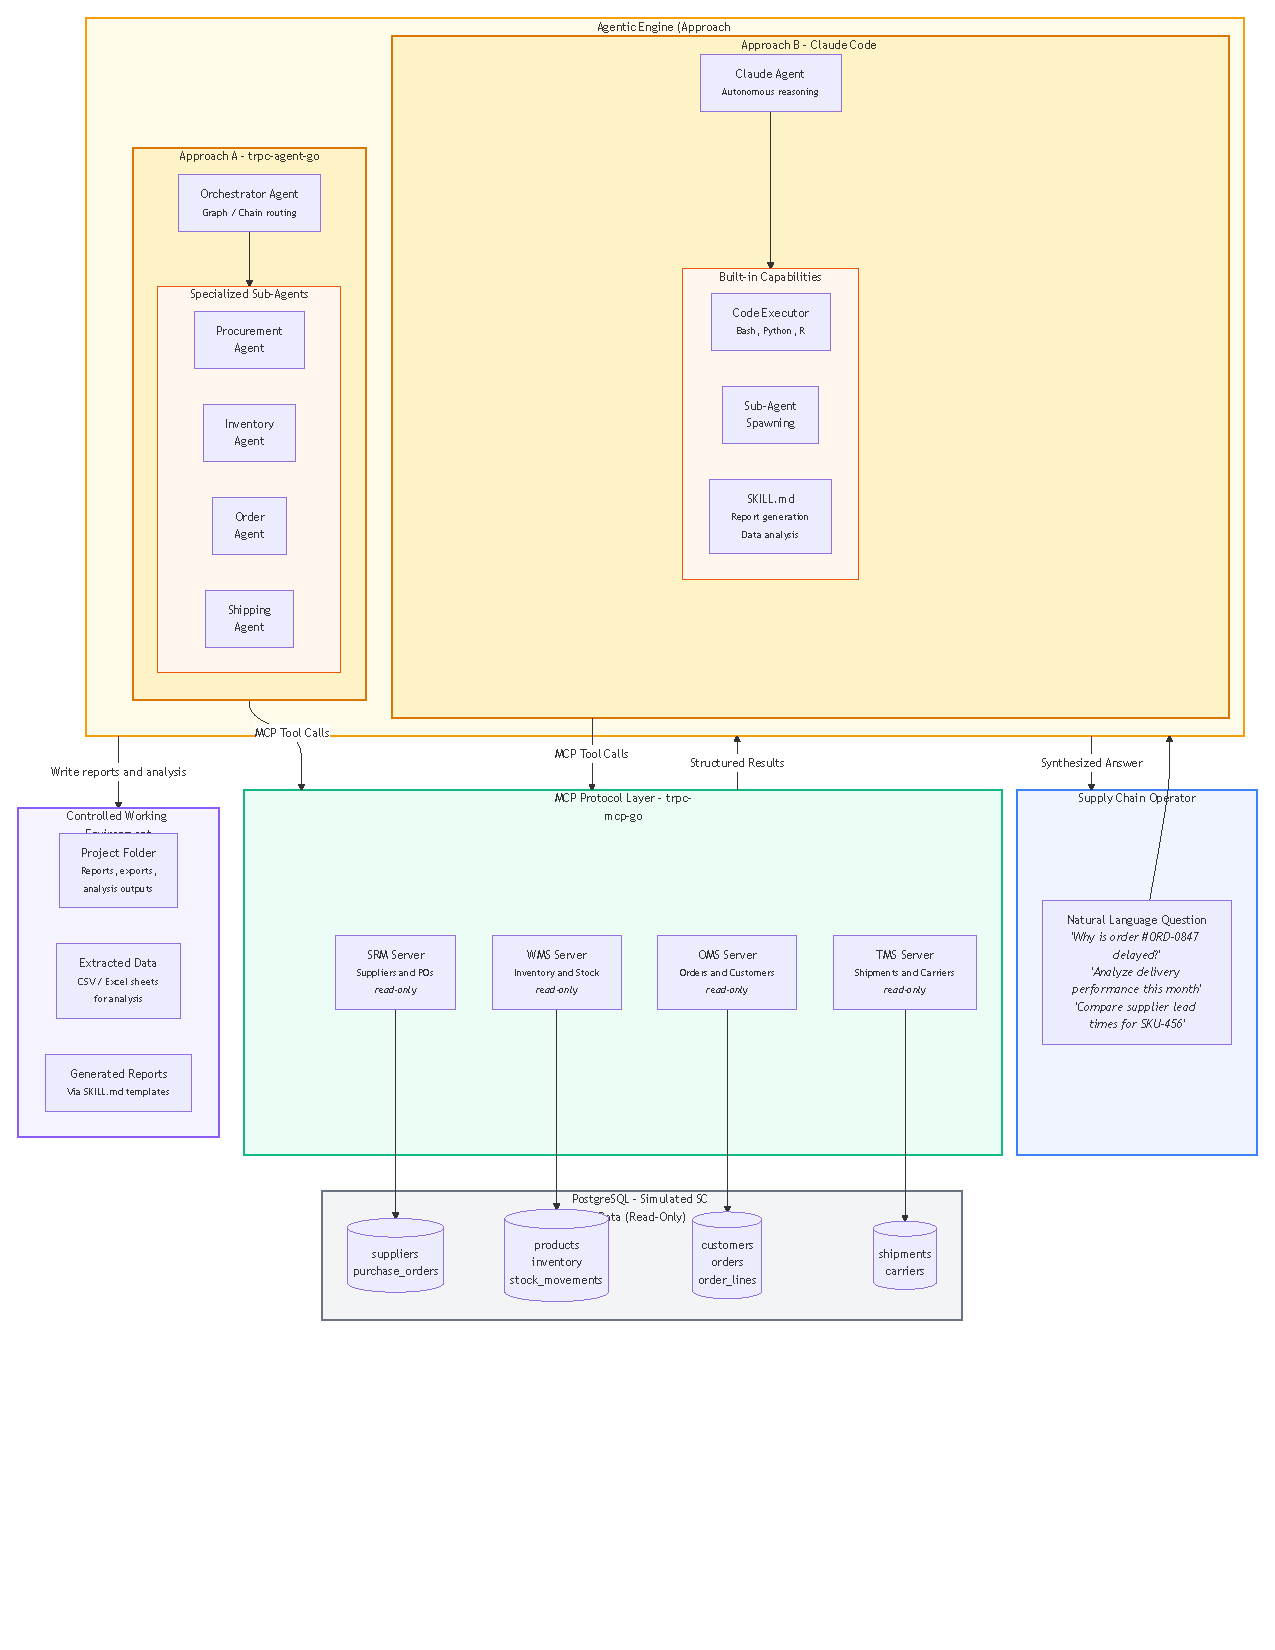
\includegraphics[width=\textwidth,height=0.85\textheight,keepaspectratio]{figures/architecture.pdf}
\caption{End-to-end architecture: two agentic approaches (trpc-agent-go \textit{or} Claude Code SDK/CLI) connecting to four read-only MCP servers, with a controlled working environment for reports and data analysis.}
\label{fig:architecture}
\end{figure}

% =====================================================================
\newpage
\section{External Data Sources: Supply Chain Systems}
% =====================================================================

\subsection{Systems We Model}

We simulate a \textbf{simplified distribution company} with four enterprise systems. These are the external data sources our agent queries through MCP. \textbf{All access is read-only.}

\begin{table}[H]
\centering\small
\begin{tabularx}{\textwidth}{@{}l l l X@{}}
\toprule
\thead{System} & \thead{Full Name} & \thead{Real-World Examples} & \thead{What It Manages} \\
\midrule
\textbf{SRM} & Supplier Relationship Mgmt & SAP Ariba, Coupa   & Suppliers, Purchase Orders, Lead Times, Performance \\
\textbf{WMS} & Warehouse Management       & SAP EWM, Manhattan  & Products, Inventory, Stock Movements, Locations \\
\textbf{OMS} & Order Management           & SAP SD, Salesforce  & Customers, Sales Orders, Order Lines, Fulfillment \\
\textbf{TMS} & Transport Management       & SAP TM, project44   & Shipments, Carriers, Tracking, Route Planning \\
\bottomrule
\end{tabularx}
\end{table}

\subsection{MCP Server Exposure (Read-Only)}

Each system is implemented as a \textbf{separate MCP server} with read-only tools:

\begin{table}[H]
\centering\small
\begin{tabularx}{\textwidth}{@{}l l X@{}}
\toprule
\thead{MCP Server} & \thead{Read-Only Tools} & \thead{Example Query} \\
\midrule
\texttt{srm-server} & \texttt{get\_supplier}, \texttt{list\_purchase\_orders}, \texttt{get\_supplier\_perf} & ``Which suppliers deliver product~X?'' \\
\texttt{wms-server} & \texttt{check\_inventory}, \texttt{get\_stock\_movements}, \texttt{get\_product} & ``Current stock of SKU-456?'' \\
\texttt{oms-server} & \texttt{get\_order}, \texttt{list\_orders\_by\_customer}, \texttt{get\_order\_lines} & ``All pending urgent orders?'' \\
\texttt{tms-server} & \texttt{get\_shipment}, \texttt{get\_carrier\_performance}, \texttt{track\_delivery} & ``Where is the shipment for order~\#123?'' \\
\bottomrule
\end{tabularx}
\end{table}

\subsection{Simulated Data Scale}

\begin{table}[H]
\centering\small
\begin{tabularx}{0.75\textwidth}{@{}l r X@{}}
\toprule
\thead{Entity} & \thead{Count} & \thead{Notes} \\
\midrule
Suppliers         & 5   & Different countries, varying reliability \\
Products          & 30  & 3 categories, fast/slow movers \\
Customers         & 50  & Retail, wholesale, enterprise segments \\
Orders            & 500 & 3 months of transactional history \\
Purchase Orders   & 100 & From various suppliers \\
Shipments         & 400 & Including exception statuses \\
Inventory Records & 60  & 30 products $\times$ 2 warehouses \\
\bottomrule
\end{tabularx}
\end{table}

\subsection{Built-In Investigation Scenarios}

We embed five realistic scenarios in the seed data. These serve both as demonstrations and as \textbf{evaluation benchmarks}: we know the correct answer for each and can measure the agent's ability to find it.

\begin{enumerate}[leftmargin=2em, itemsep=0.5em]
    \item \textbf{Stockout Investigation:} Product has 0~inventory; orders unfulfilled; purchase order delayed from supplier. Agent must connect WMS $\to$ OMS $\to$ SRM.
    \item \textbf{Late Delivery:} Urgent customer order; shipment in ``exception'' status; carrier with poor on-time rate. Agent must connect OMS $\to$ TMS.
    \item \textbf{Supplier Comparison:} Same product from 2 suppliers with different lead times, costs, reliability. Agent must query SRM and cross-reference with WMS receiving history.
    \item \textbf{Demand Spike:} Sudden order surge depleting inventory faster than the reorder point predicted. Agent must analyze OMS trends and WMS levels.
    \item \textbf{Cross-Warehouse Transfer:} Product available in WH-B but customer is near WH-A. Agent must check WMS for both warehouses and TMS for shipping options.
\end{enumerate}

% ── Data Model (full page) ───────────────────────────────────────────
\newpage
\subsection{Data Model}

\begin{figure}[H]
\centering
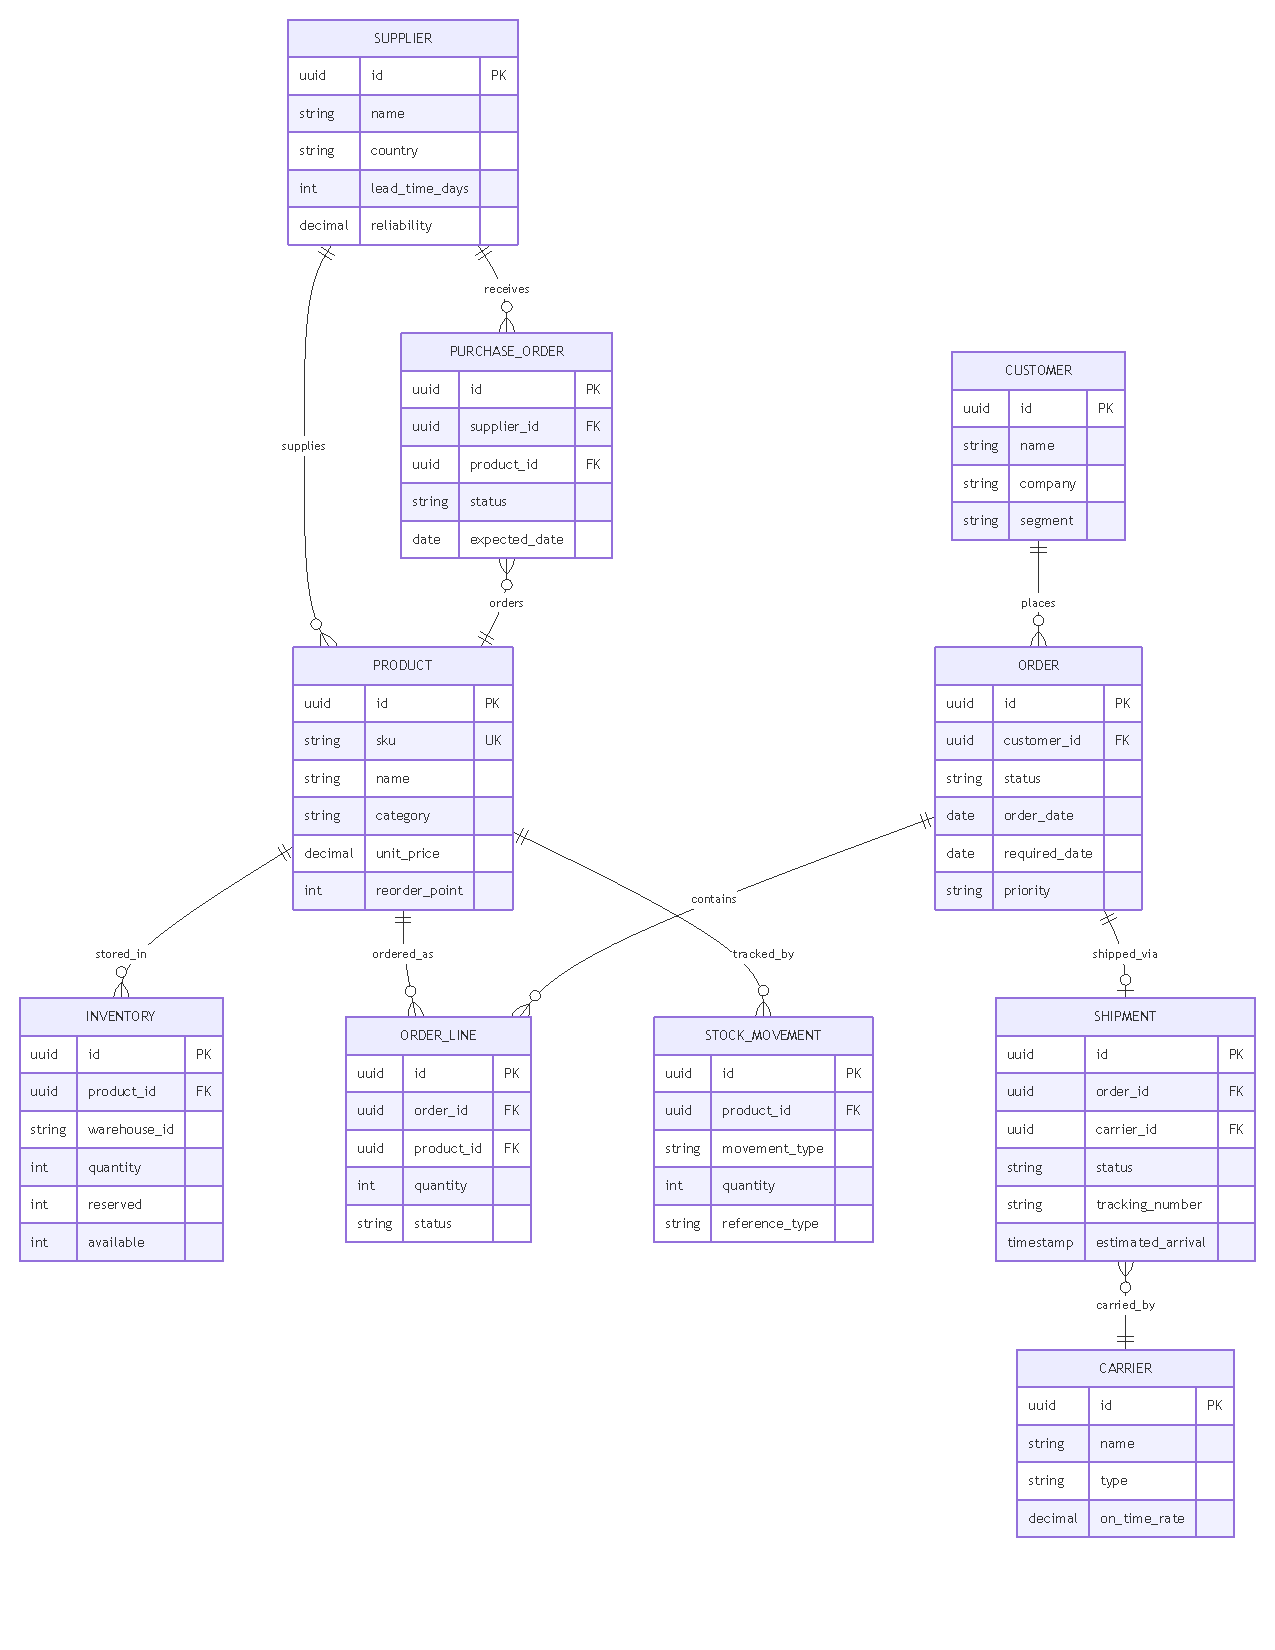
\includegraphics[width=\textwidth,height=0.88\textheight,keepaspectratio]{figures/data_model.pdf}
\caption{Entity-relationship diagram: cross-system data model spanning SRM, WMS, OMS, and TMS.}
\label{fig:data-model}
\end{figure}

% =====================================================================
% ── GANTT CHART (landscape, full page) ───────────────────────────────
% =====================================================================
\newpage
\section{Project Timeline}

The project spans \textbf{8~weeks} (February~5 -- April~15,~2026), organized into five parallel workstreams.

\begin{landscape}
\thispagestyle{empty}
\vspace*{\fill}
\begin{figure}[H]
\centering
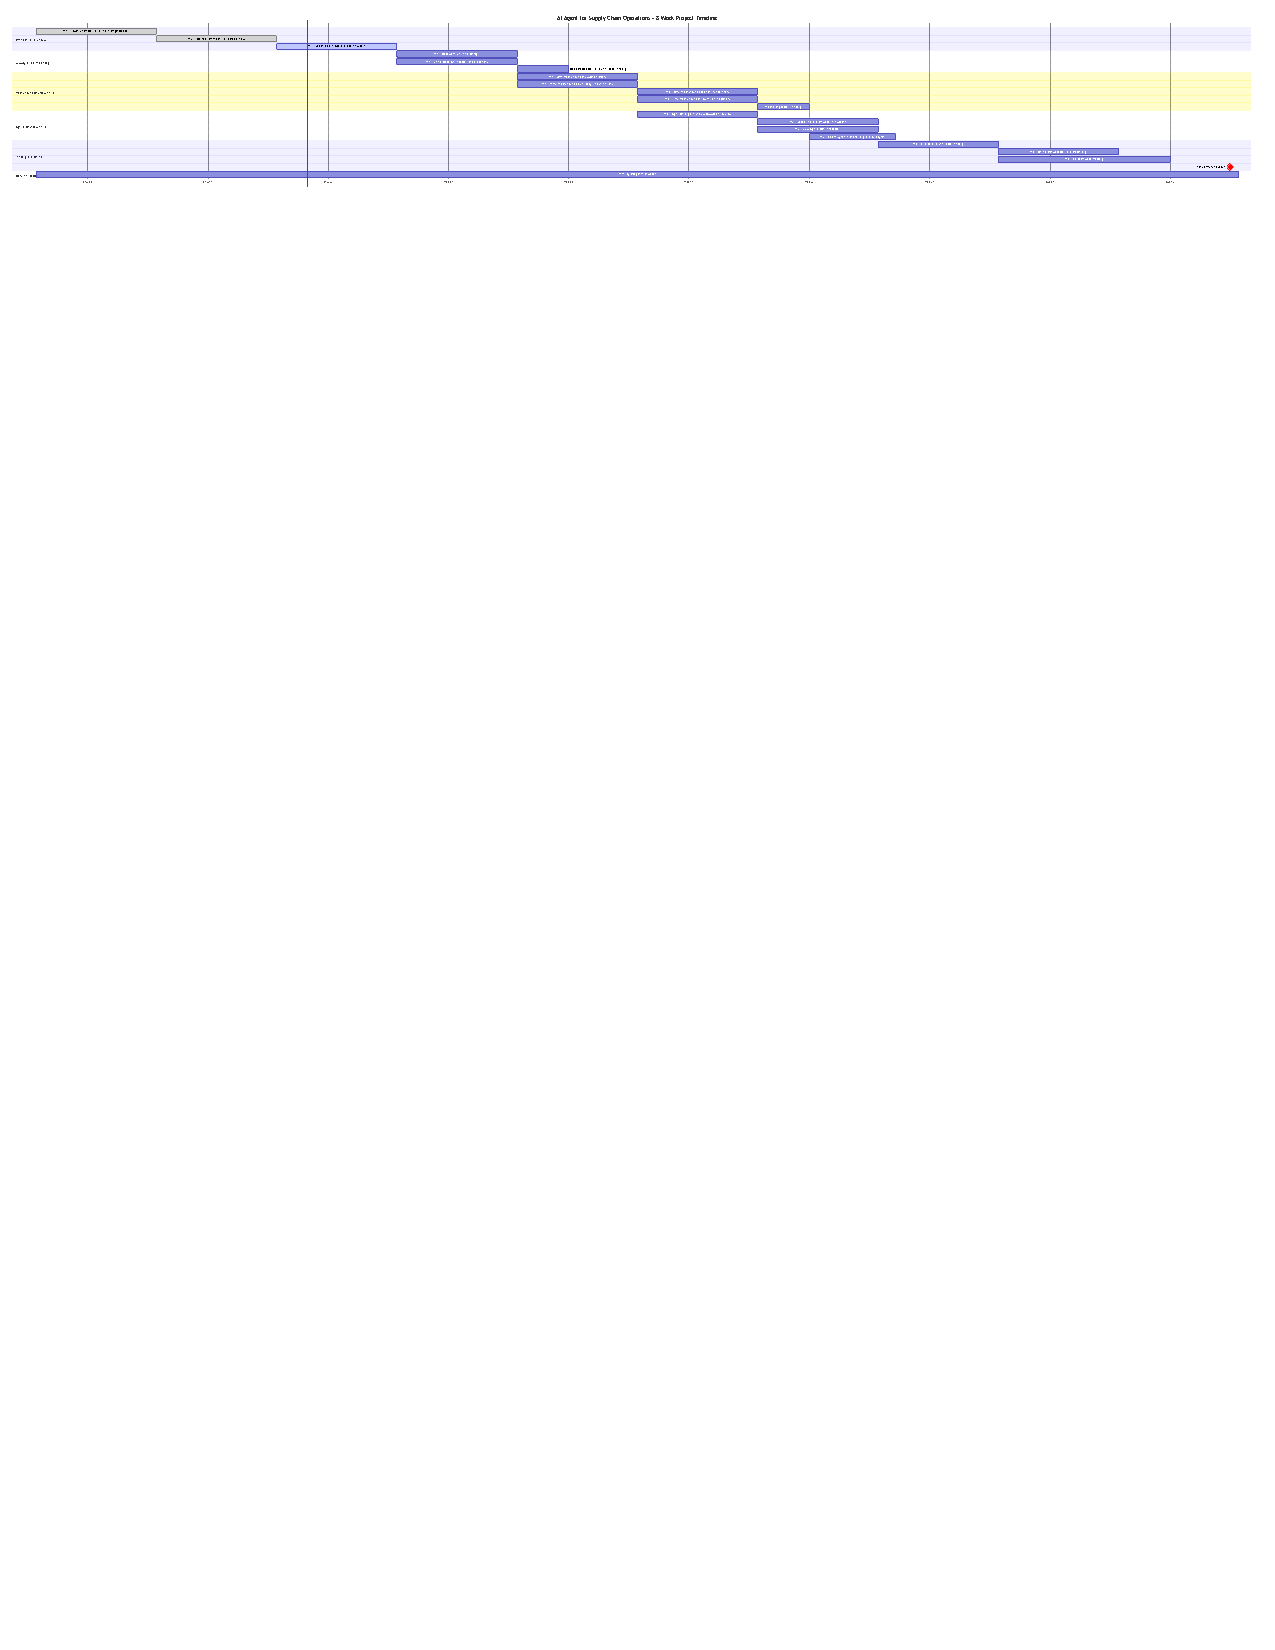
\includegraphics[width=\linewidth]{figures/gantt.pdf}
\caption{8-week Gantt chart: from research through final presentation on April~15, 2026.}
\label{fig:gantt}
\end{figure}
\vspace*{\fill}
\end{landscape}

\subsection{Week-by-Week Summary}

\begin{table}[H]
\centering\small
\begin{tabularx}{\textwidth}{@{} c l l X @{}}
\toprule
\thead{Week} & \thead{Dates} & \thead{Focus} & \thead{Deliverable} \\
\midrule
1 & Feb 5--11   & Topic Selection \& Registration & Project proposal \\
2 & Feb 12--18  & Domain Research \& Roadmap      & Progress report, roadmap \\
3 & Feb 19--25  & State of the Art \& Frameworks  & Literature review, framework analysis \\
4 & Feb 26--Mar 4 & Database Schema \& Data Gen.  & PostgreSQL schema, seed scripts \\
5 & Mar 5--11   & MCP Servers (SRM, WMS)           & Working read-only MCP servers for 2~systems \\
6 & Mar 12--18  & MCP Servers (OMS, TMS) + Agent   & All 4 MCP servers, agent scaffolding, skills \\
7 & Mar 19--25  & Agent Integration \& Reasoning   & Working agent, sub-agents, data analysis \\
8 & Mar 26--Apr 15 & Testing, Demo \& Final Report & Scenario evaluation, presentation, report \\
\bottomrule
\end{tabularx}
\end{table}

% =====================================================================
\newpage
\section{Next Steps}
% =====================================================================

\begin{itemize}[itemsep=0.6em]
    \item \textbf{This week (W3):} Finalize literature review; validate framework selection with tutor.
    \item \textbf{Next week (W4):} Begin PostgreSQL schema implementation for all four systems; write seed data generation scripts with embedded investigation scenarios.
    \item \textbf{Ongoing:} Continue contributions to the \texttt{trpc-agent-go} open-source project.
\end{itemize}

% =====================================================================
\newpage
\section{Bibliography}
% =====================================================================

\renewcommand{\arraystretch}{1.25}
\begin{enumerate}[leftmargin=2em, itemsep=0.4em, label={[\arabic*]}]
    \item Jannelli, V., Schoepf, S., Bickel, M., Netland, T., \& Brintrup, A. (2024). Agentic LLMs in the Supply Chain: Towards Autonomous Multi-Agent Consensus-Seeking. \textit{arXiv:2411.10184}. Published in \textit{Int.\ J.\ Production Research}, 2025. \href{https://arxiv.org/abs/2411.10184}{arXiv}

    \item Yin, J. et al. (2025). Rethinking Supply Chain Planning: A Generative Paradigm. \textit{arXiv:2509.03811}. \href{https://arxiv.org/abs/2509.03811}{arXiv}

    \item AlMahri, S., Xu, L., \& Brintrup, A. (2026). Automating Supply Chain Disruption Monitoring via an Agentic AI Approach. \textit{arXiv:2601.09680}. \href{https://arxiv.org/abs/2601.09680}{arXiv}

    \item Yoshizato, K. et al. (2026). AI Agent Systems for Supply Chains: Structured Decision Prompts and Memory Retrieval. \textit{arXiv:2602.05524}. Accepted at AAMAS~2026. \href{https://arxiv.org/abs/2602.05524}{arXiv}

    \item Quan, Y. \& Liu, Z. (2024). InvAgent: A LLM-based Multi-Agent System for Inventory Management. \textit{arXiv:2407.11384}. \href{https://arxiv.org/abs/2407.11384}{arXiv}

    \item Gosmar, D. et al. (2025). Agentic AI Sustainability Assessment for SC Document Insights. \textit{arXiv:2511.07097}. \href{https://arxiv.org/abs/2511.07097}{arXiv}

    \item Zhang, Y. et al. (2025). From Unstructured Communication to Intelligent RAG: Multi-Agent Automation for Supply Chain Knowledge Bases. \textit{arXiv:2506.17484}. KDD~2025 Workshop. \href{https://arxiv.org/abs/2506.17484}{arXiv}

    \item Parekh, R. et al. (2025). Leveraging Knowledge Graphs and LLM Reasoning to Identify Operational Bottlenecks for Warehouse Planning. \textit{arXiv:2507.17273}. \href{https://arxiv.org/abs/2507.17273}{arXiv}

    \item Integrating RAG with Prompt Engineering for Knowledge-Driven SC Solutions. (2025). \textit{ResearchGate Publication~393479215}. \href{https://www.researchgate.net/publication/393479215}{ResearchGate}

    \item Zheng, G. et al. (2025). LLMs in SCM: Opportunities and a Case Study. \textit{IFAC-PapersOnLine}, MIM~2025. \href{https://www.sciencedirect.com/science/article/pii/S2405896325012595}{ScienceDirect}

    \item Li, B. et al. (2023). Large Language Models for Supply Chain Optimization (OptiGuide). \textit{arXiv:2307.03875}. \href{https://arxiv.org/abs/2307.03875}{arXiv}

    \item Enhancing SC Resilience with Multi-Agent Systems and Machine Learning. (2025). \textit{Am.\ J.\ Eng.\ \& Tech.} \href{https://theamericanjournals.com/index.php/tajet/article/view/5919}{Journal}

    \item Intelligent Human-Machine Partnership for Manufacturing: Simulation-Driven KGs and LLM Collaboration. (2025). \textit{arXiv:2512.18265}. \href{https://arxiv.org/abs/2512.18265}{arXiv}

    \item Supply Chain Mapping through RAG: Applications to the Electronics Industry. (2026). \textit{J.\ Operational Research Society}. \href{https://www.tandfonline.com/doi/full/10.1080/01605682.2025.2608868}{Taylor \& Francis}
\end{enumerate}
\renewcommand{\arraystretch}{1.0}

\end{document}
